\documentclass[12pt]{article}

% Any percent sign marks a comment to the end of the line

% Every latex document starts with a documentclass declaration like this
% The option dvips allows for graphics, 12pt is the font size, and article
%   is the style


\usepackage{url}
\usepackage{graphicx}
\usepackage{subcaption}

% These are additional packages for "pdflatex", graphics, and to include
% hyperlinks inside a document.


\addtolength{\oddsidemargin}{-.875in}
\addtolength{\evensidemargin}{-.875in}
\addtolength{\textwidth}{1.75in}

\addtolength{\topmargin}{-.875in}
\addtolength{\textheight}{1.75in}

% These force using more of the margins that is the default style

\begin{document}

% Everything after this becomes content
% Replace the text between curly brackets with your own

\title{Team 07 - Update 1 \\
	   \large CS6220 - Data Mining Techniques - Fall 2017 \\
	   \large Northeastern University}
\author{Nakul Camasamudram, Rosy Parmar, Rahul Verma, Guiheng Zhou}
\date{\today}



\maketitle

% This command causes the title to be created in the document
\section{Introduction}
Our team is using "The Instacart Online Grocery Shopping Dataset 2017" to build a Recommender System. \\ 
Instacart is an American company that operates as a same-day grocery delivery service. This anonymized dataset contains a sample of over 3 million grocery orders from more than 200,000 Instacart users, spread over 6 .csv files. For each user, the dataset has 4 to 100 of their orders, with the sequence of products purchased in each order. The week and hour of the day the order was placed, and a relative measure of time between orders is also available.

\section{Data Analysis}

\subsection{The Dataset}

Orders from Instacart are available in four .csv files: "orders.csv", "order\_products\_\_train.csv", "order\_products\_\_prior.csv" and "sample\_submission.csv". The key to understand the dataset and the train / test split is the orders table ("orders.csv").

Take for example User 1[Fig 1] , who happens to be a train user. User 1 has 10 prior orders, and 1 train order whose details are provided in "order\_products\_\_prior.csv" and in "order\_products\_\_train.csv" respectively.

\begin{figure}[!bp]
  \begin{subfigure}[b]{0.4\textwidth}
    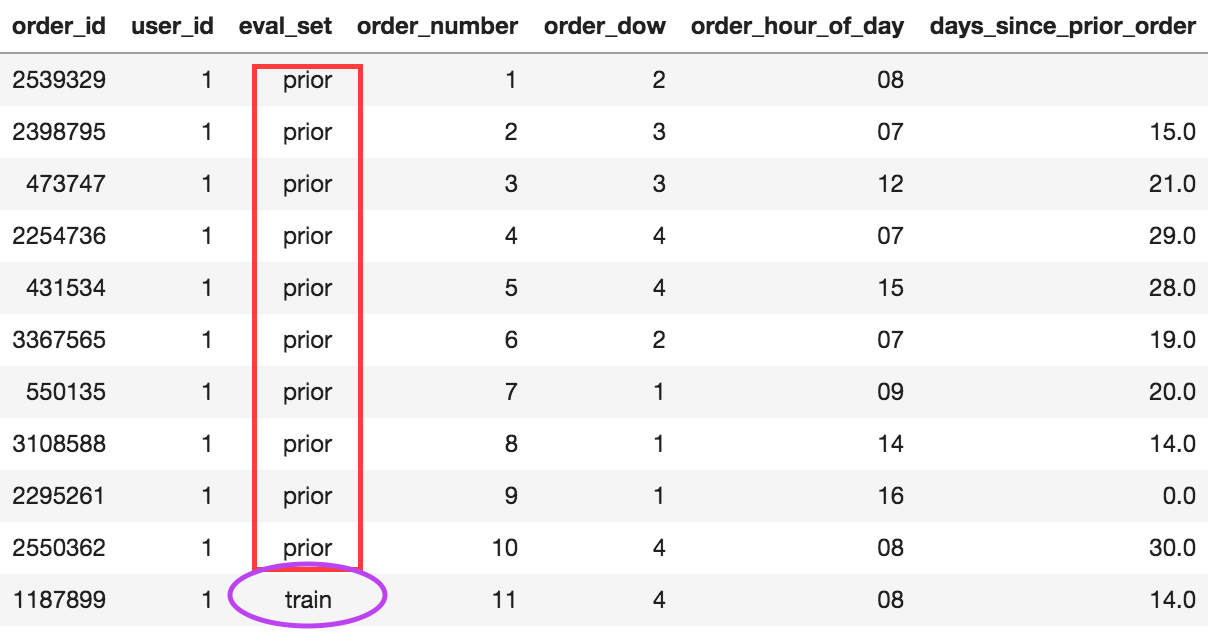
\includegraphics[width=\textwidth]{train_user.png}
    \caption{User 1}
    \label{fig:f1}
  \end{subfigure}
  \hfill
  \begin{subfigure}[b]{0.4\textwidth}
    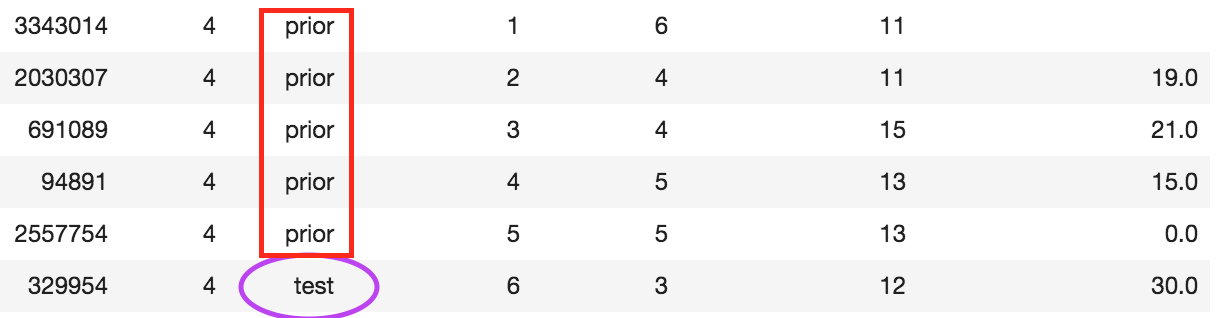
\includegraphics[width=\textwidth]{test_user.png}
    \caption{User 4}
    \label{fig:f2}
  \end{subfigure}
  \caption{Train/Test Split}
\end{figure}

Similarly, User 4 is a test user. He has 5 prior orders, and his 6th is a test order. Their details are available in "order\_products\_\_prior.csv" and "sample\_submission.csv" respectively.

Figure 2 is a glimpse at "order\_products\_\_prior.csv" when merged with three other .csv files that represent products, aisles and departments. The format of "sample\_submission.csv" and "order\_products\_\_train.csv" is exactly the same.

\begin{figure*}
	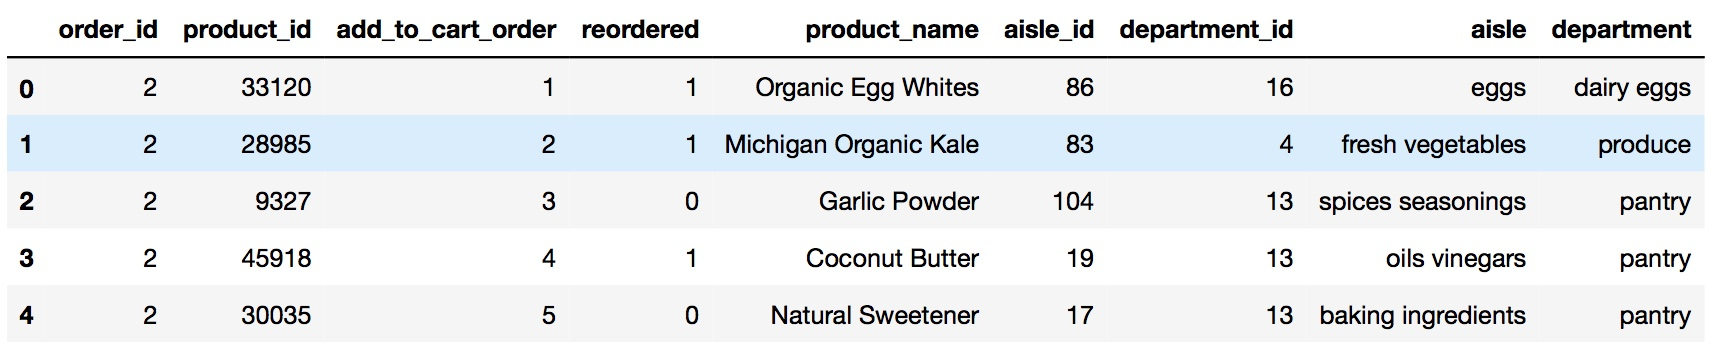
\includegraphics[scale=0.3]{prior_df_merged} \\
	\caption{Merged Prior Orders}
\end{figure*}


\subsection{Exploration and Analysis}

\noindent
\textbf{How many orders have users placed?} \\
The below histogram validates the claim that 4 to 100 orders of a customer are given.
\begin{center}
	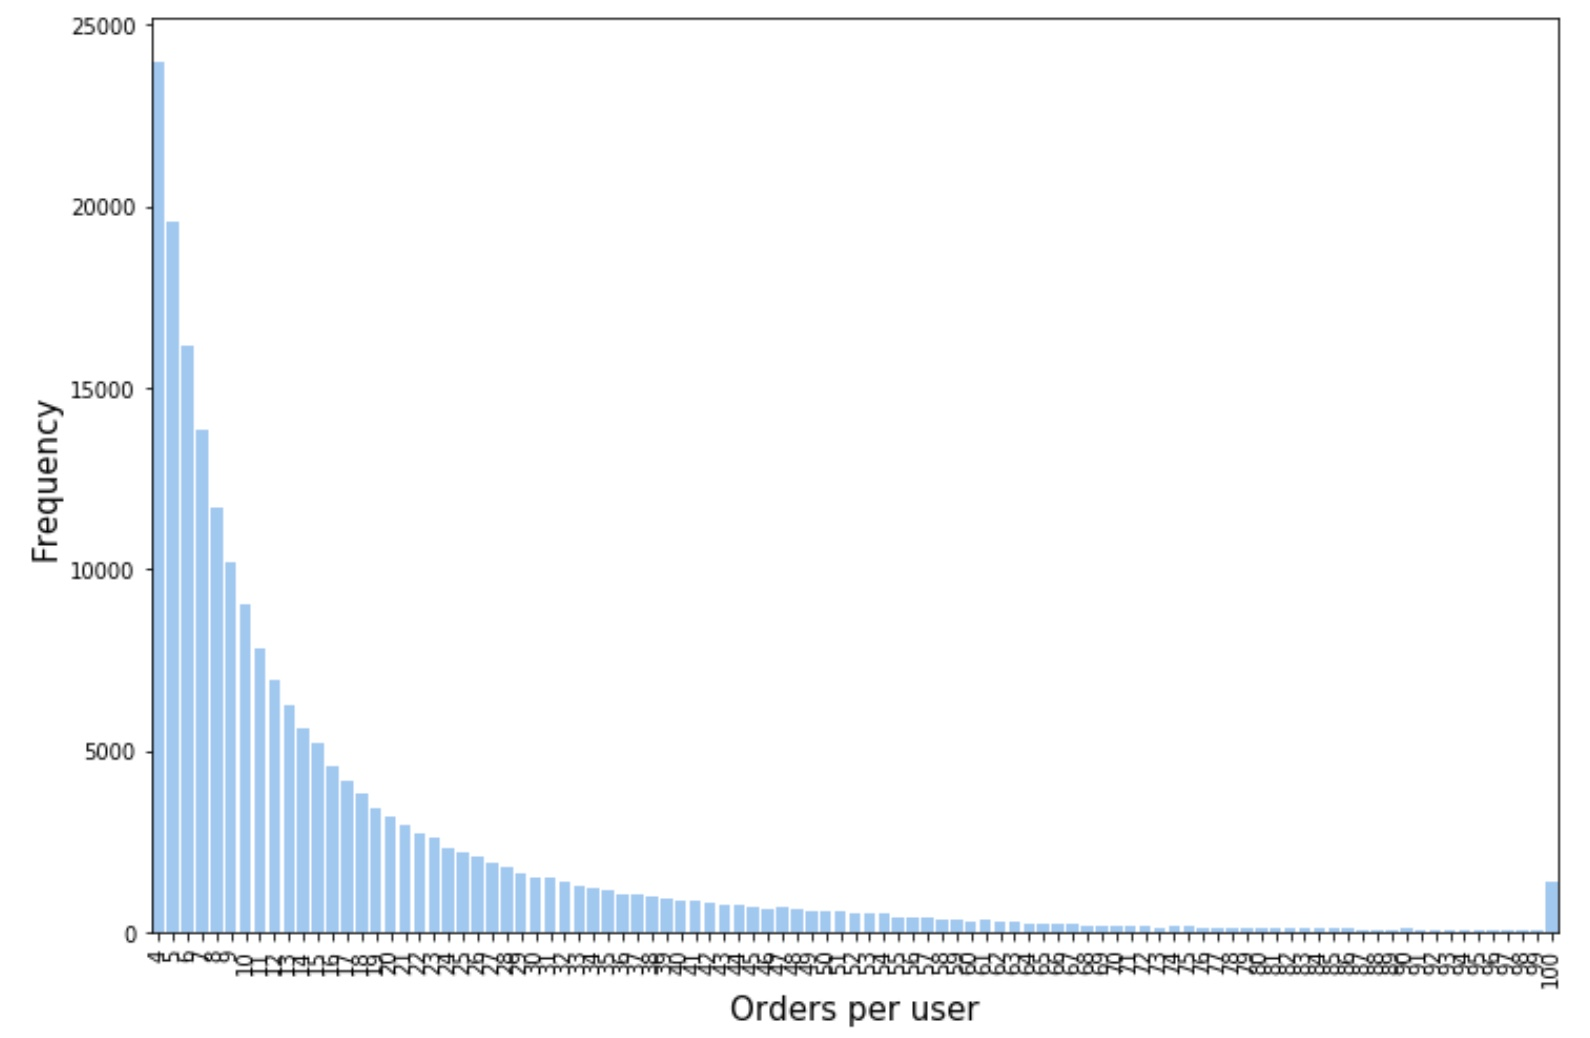
\includegraphics[scale=0.2]{order_user}
\end{center}


\noindent
\textbf{How many products does an order have??} \\
The "long tail" phenomenon is clearly visible here.
\begin{center}
	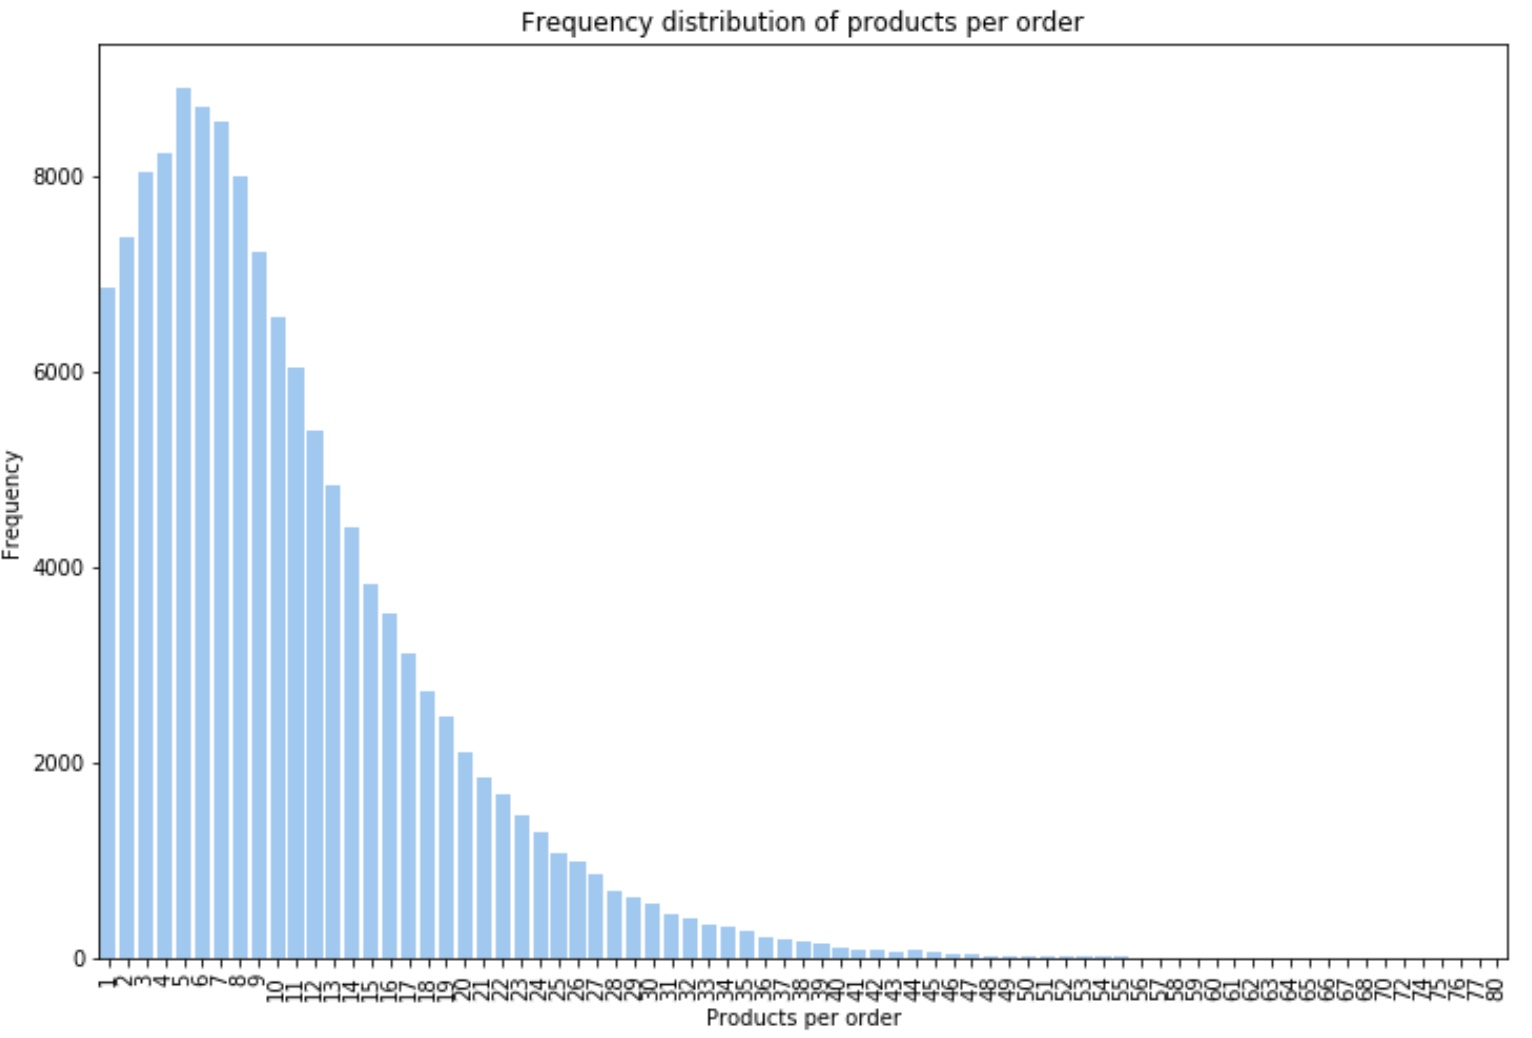
\includegraphics[scale=0.2]{train_products_order}
\end{center} 

\noindent
\textbf{Does day of the week influence user order habits?} \\
There is a clear effect of day of the week. Most orders are on days 0 and 1. However, there is no information about which values represent which day, but, it's reasonable to assume they are weekends.
\begin{center}
	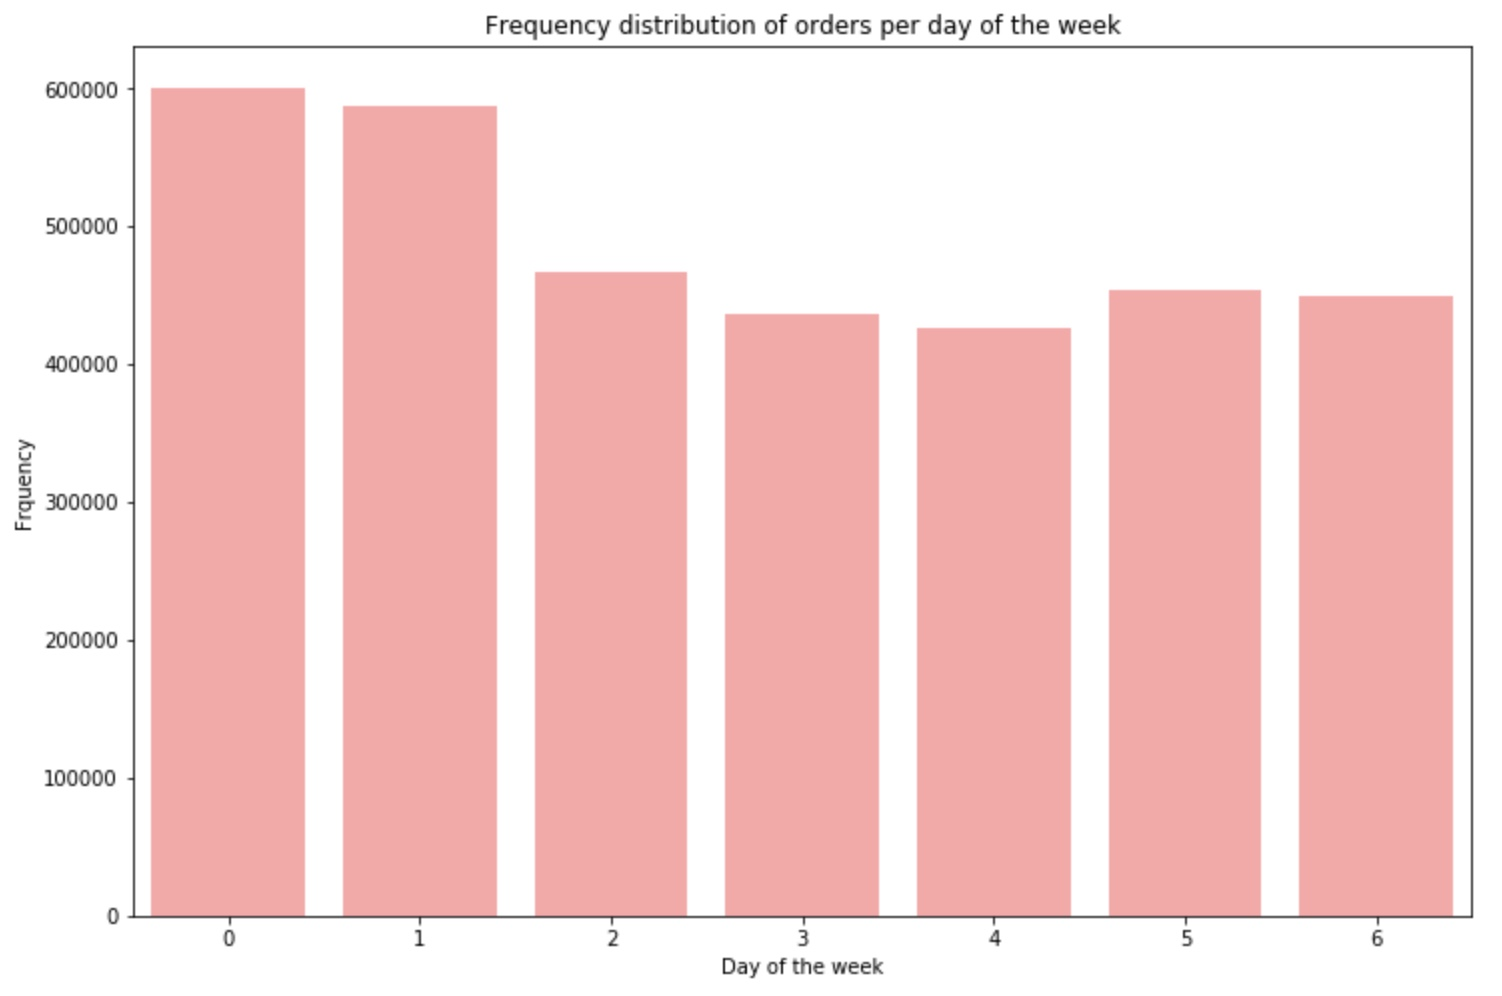
\includegraphics[scale=0.2]{order_dow}
\end{center}

\noindent
\textbf{Does time of day influence user order habits?} \\
There is a clear effect. Most of the orders are placed between 7.00 am and 10.00pm.
\begin{center}
	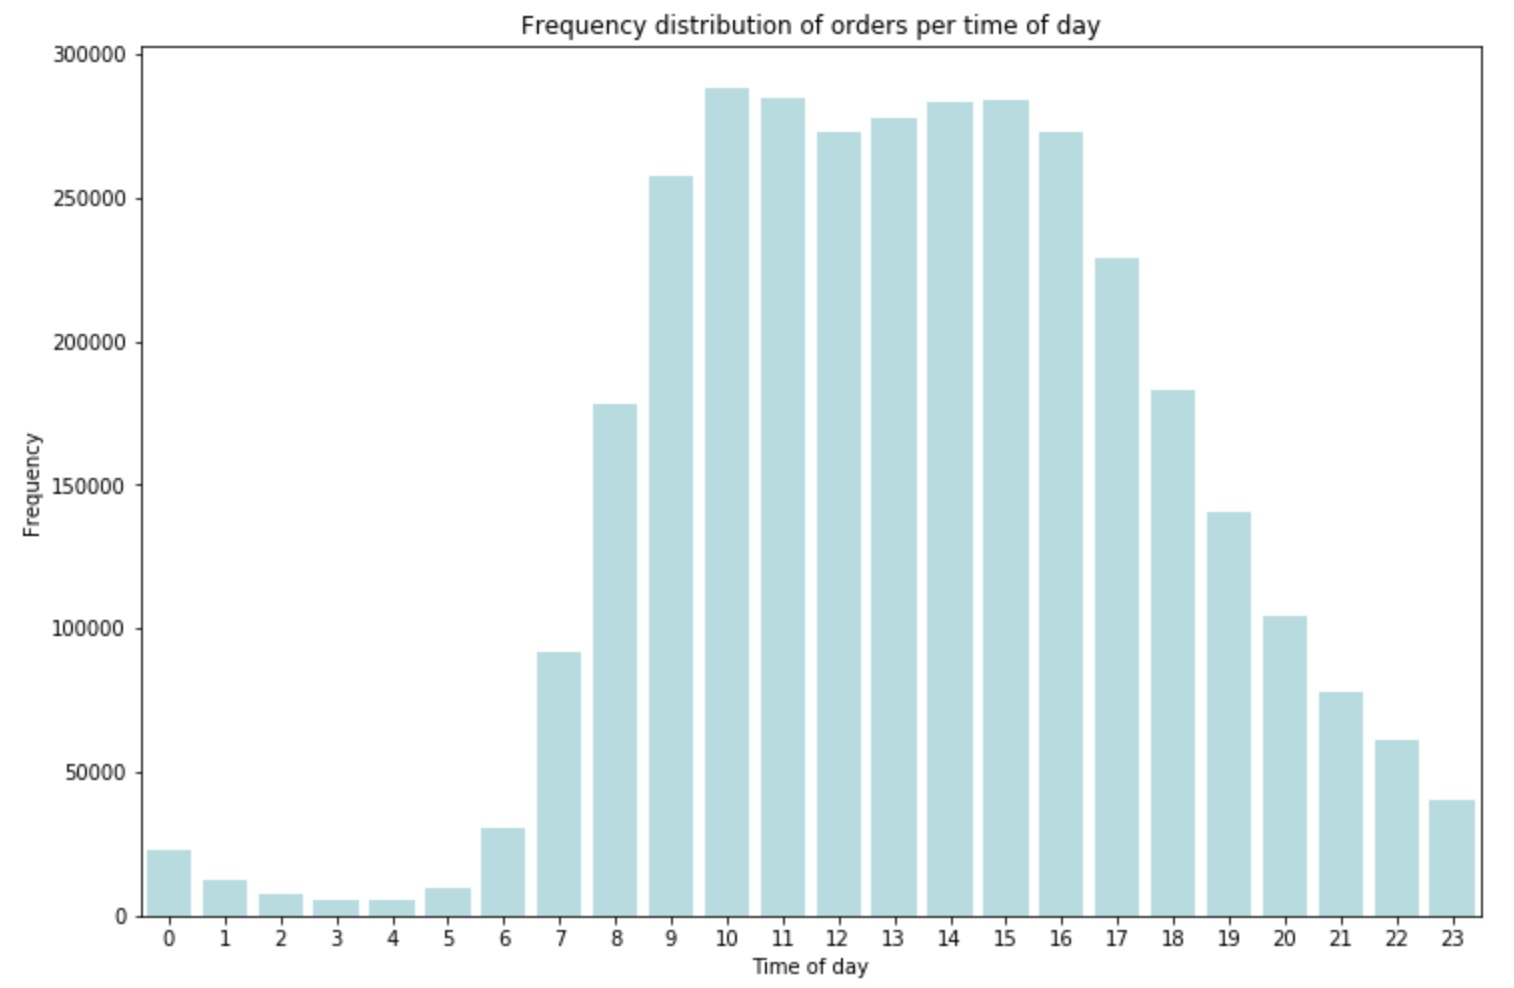
\includegraphics[scale=0.2]{order_tod}
\end{center}

\noindent
\textbf{When do users reorder?} \\
Users seem to order on a weekly and monthly basis.
\begin{center}
	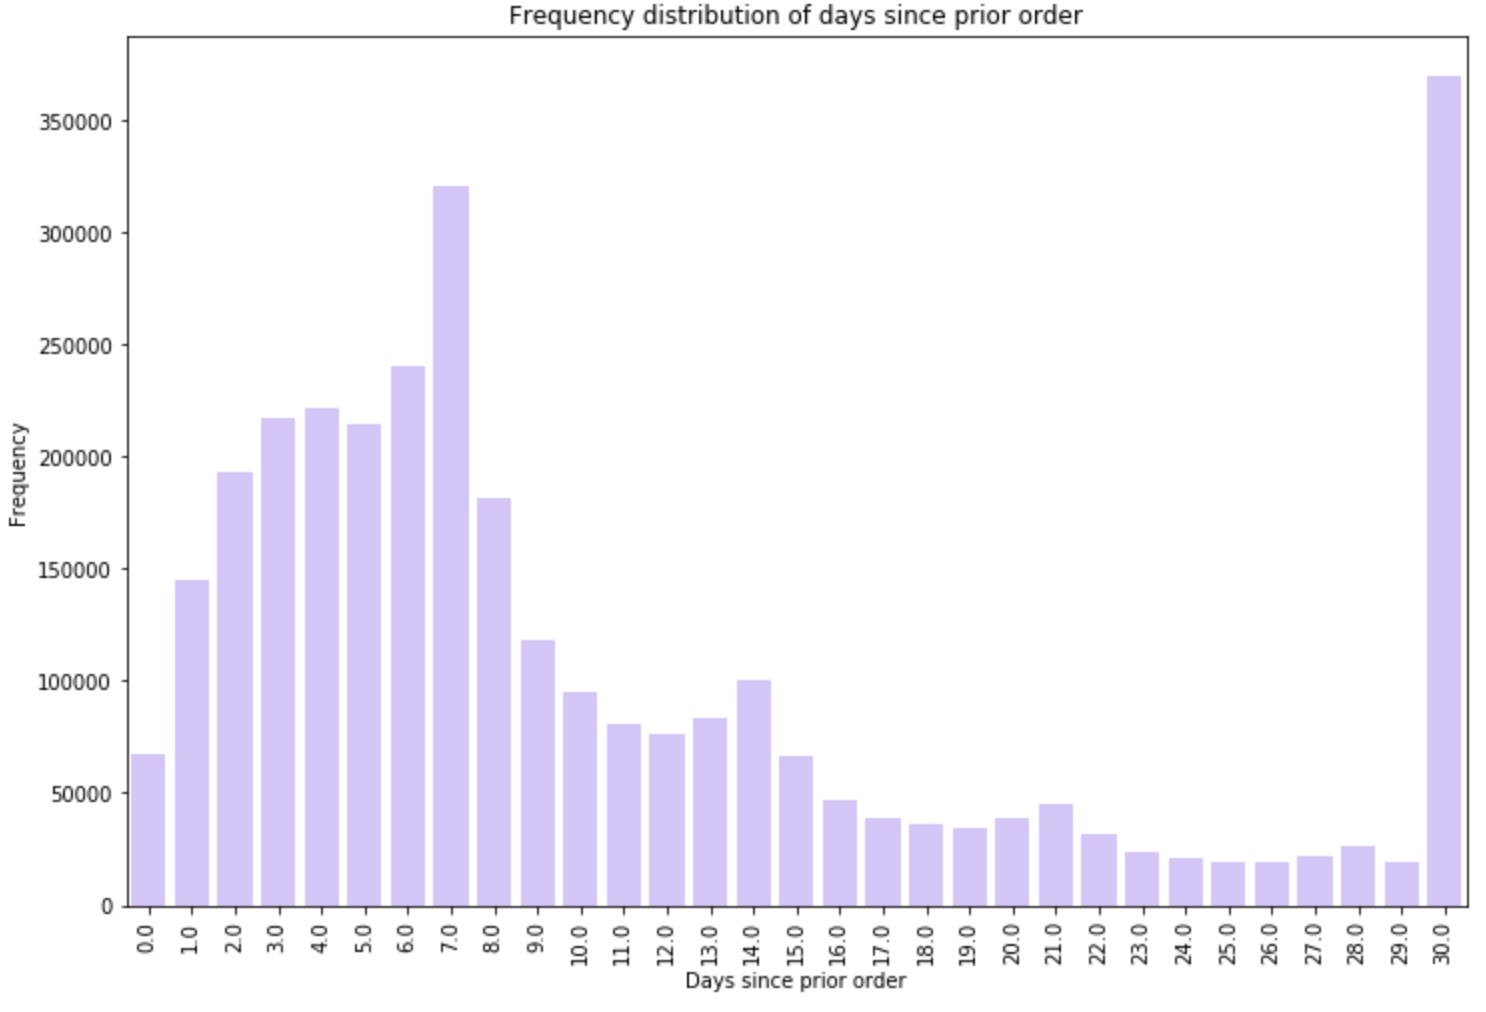
\includegraphics[scale=0.2]{days_since_prior_order}
\end{center}


\noindent
\textbf{What are the top 20 Products?} \\
\begin{center}
	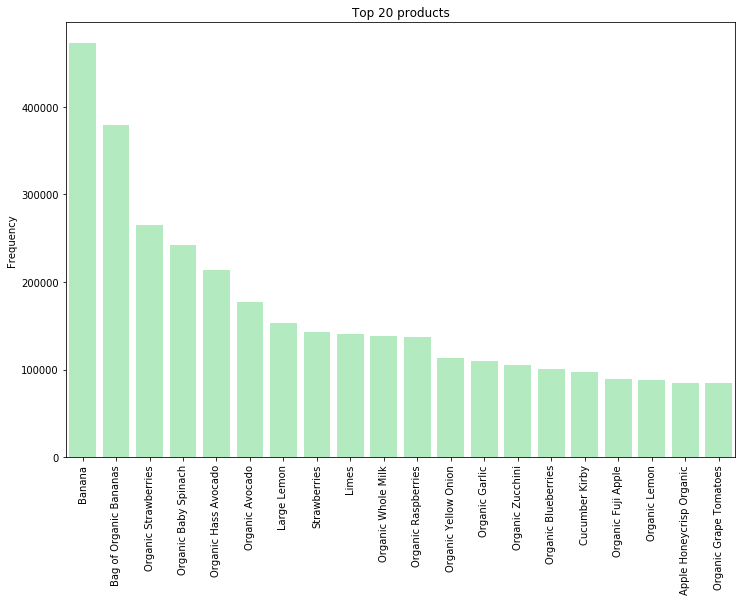
\includegraphics[scale=0.4]{top_20_products.png}
\end{center}


\section{Next Steps}
We will be following a Collaborative Filtering based approach to build our recommender system. We initially decided against at a content-based approach since our dataset does not have enough metadata information to profile each product. \\

Roughly, these are the steps we'd like to follow

\begin{itemize}
	\item Represent the given data in the form of a $user \times products$ matrix, where each entry would represent frequency of product purchase by a certain user. 
	\item Normalize each entry in the matrix to fit into 0-1 range.
	\item Explore three algorithms either separately or in combination: User/Item based Collaborative Filtering, Matrix Factorization and Association Rules.
	\item For every model above, validate it against the test set using the F1 measure as an accuracy metric.
	\item Evaluate models by comparing them against a baseline model which returns the most popular products.
\end{itemize}

\end{document}





















